\section{Introducción}
La planificación de la producción es una disciplina clave en la gestión de 
activos y se utiliza para determinar la forma más eficiente de asignar 
recursos, como maquinaria, mano de obra y tiempo, con el fin de alcanzar 
los objetivos de producción. Es un proceso que implica la toma de decisiones 
sobre qué recursos, cuánto, cuándo y cómo producirlos, con el objetivo de optimizar la 
utilización de los elementos disponibles, maximizando la eficiencia y rentabilidad 
del proceso de producción. La planificación de la producción se aplica en una 
amplia gama de sectores y áreas de negocio, incluyendo la fabricación, la logística, 
el transporte, la distribución y la gestión de la cadena de suministro, entre otros.\medskip

La importancia de la planificación de la producción radica en su capacidad para mejorar 
la eficiencia mediante una buena gestión de las operaciones, lo que puede tener un impacto 
significativo en la rentabilidad y competitividad de las empresas. Una planificación de 
producción efectiva debe optimizar la asignación de recursos, minimizar los tiempos de 
inactividad, reducir los costos de producción y maximizar el cumplimiento de los plazos 
de entrega en la medida de lo posible. Esto lo que resulta es en una mayor eficiencia operativa 
y una mejor calidad del producto o servicio.\medskip

Sin embargo, la planificación de la producción es un problema complejo debido a la gran 
cantidad de variables y restricciones que deben tenerse en cuenta, como los tiempos de 
procesamiento, las capacidades de los recursos, las restricciones de almacenamiento y 
transporte y las demandas de los clientes, entre otros. Tradicionalmente el Job Shop Scheduling 
Problem (JSP) y el Flexible Shop Scheduling Problem (FJSP) \cite{FJSP-article} se ha abordado 
utilizando enfoques heurísticos y metaheurísticos. Estos problemas de optimización combinatorios 
son muy conocidos dentro del los problemas NP-Hard \cite{Derivando_2017}, que son aquellos para 
los que no existen algoritmos eficientes para encontrar soluciones óptimas en un 
tiempo razonable.\medskip

Un problema NP-Hard es un tipo de problema de optimización en el cual no se conocen algoritmos 
exactos que puedan encontrar una solución óptima en un tiempo polinómico. Esto implica que a 
medida que el tamaño del problema aumenta, el tiempo de cómputo necesario para encontrar una 
solución óptima también se vuelve prohibitivamente alto. Estos problemas son considerados de 
gran complejidad y representan un desafío significativo para la investigación en ciencias de 
la computación. La importancia de identificar un problema como NP-Hard radica en que a menudo 
técnicas utilizadas para un problema pueden ser aplicados a otros problemas NP-Hard. Esto se debe a que 
muchos problemas NP-Hard comparten estructuras y patrones similares, lo que permite la 
transferencia de conocimientos y técnicas de un problema a otro. Por lo tanto, encontrar 
soluciones eficientes o aproximadas para un problema NP-Hard particular puede tener un impacto 
significativo en la resolución de otros problemas que enfrentan desafíos similares.\medskip

En los últimos años, ha surgido el Imitation Learning (IL) \cite{SmartLab_2019} como una 
prometedora técnica de aprendizaje automático. El IL se basa en el concepto de aprender 
de la experiencia de expertos humanos o de sistemas previamente establecidos, y luego utilizar 
ese conocimiento para guiar la toma de decisiones en situaciones similares. Esto se puede lograr 
a través de enfoques supervisados, donde se entrena a un modelo para imitar las acciones de 
expertos humanos, o a través de enfoques de Reinforcement Learning (RL) \cite{Bhatt_2018}, 
donde se permite que un modelo aprenda a partir de la retroalimentación y la interacción 
con el entorno.\medskip

En este contexto, el presente trabajo se enfoca en el desarrollo de un sistema de planificación 
basado en IL, utilizando técnicas de aprendizaje supervisado y RL para resolver el FJSP. 
Se busca explorar cómo estas técnicas pueden aplicarse a la planificación de la producción, teniendo 
en cuenta los desafíos y la complejidad de este problema. A través del estudio y análisis de 
diferentes enfoques y metodologías, se pretende contribuir al campo de la planificación de la 
producción utilizando técnicas de inteligencia artificial y aprendizaje automático, con el objetivo 
de mejorar la eficiencia y la toma de decisiones en procesos industriales.

\subsection{Motivación}
Como una persona apasionada por los retos, encuentro que la planificación de la producción es un desafío 
muy estimulante dentro del marco de la industria. Me fascina la idea de que mis decisiones puedan tener un 
impacto significativo en la eficiencia, productividad y rentabilidad de los procesos de fabricación. Sin embargo, 
soy consciente de que los problemas que enfrentamos en la planificación de la producción, como el JSP y el FJSP, 
son conocidos por su alta complejidad y la falta de métodos de resolución eficientes, lo cual representa 
un mayor desafío.\medskip

Para superar estos desafíos, creo firmemente en la importancia de encontrar soluciones innovadoras y eficientes. 
Me entusiasma la aplicación de enfoques de inteligencia artificial, ya que he presenciado cómo han ganado 
cada vez más importancia en los últimos años. Estas técnicas tienen un potencial asombroso para encontrar 
soluciones aproximadas en tiempo real y adaptarse a entornos dinámicos, lo cual es realmente emocionante 
para alguien como yo, que disfruta de los retos y de encontrar soluciones creativas.\medskip

La motivación detrás de mi proyecto actual se basa en la necesidad de desarrollar enfoques de IL,
una rama del aprendizaje automático que se basa en la imitación de comportamientos de expertos,
ya que se han demostrado prometedores resultados en otros campos en los que se han aplicado. 
Además, las soluciones que se desarrollen el contexto del JSP y el FJSP podrían tener aplicaciones 
más amplias en otros problemas NP-Hard que enfrenta la industria. Desde la logística hasta la 
programación de tareas o la asignación de recursos, veo un potencial significativo 
para impactar la optimización de procesos y la competitividad de las empresas en la industria.

\subsection{Explicación del problema}
El FJSP es un desafío de optimización combinatoria que se encuentra en el campo de la la gestión de la 
producción. En este problema, se busca determinar la secuencia óptima de operaciones a realizar en una 
serie de máquinas, con el objetivo de minimizar el tiempo total de producción o maximizar la eficiencia 
del sistema. A diferencia del JSP, en el que cada operación tiene una ruta de procesamiento fija, 
las operaciones pueden ser procesadas en varias máquinas diferentes. Además, adicionalmente las 
operaciones están agrupadas dentro de un trabajo, que es un conjunto de operaciones que deben 
ser procesadas en una secuencia específica.\medskip

Existen dos restricción temporales que especifican cuándo puede comenzar 
cada operación: una operación no puede comenzar hasta que se hayan completado todas las operaciones
anteriores de la misma tarea y no puede comenzar hasta que se hayan completado todas las operaciones
anteriores de la misma máquina. El objetivo del problema es asignar las operaciones a las máquinas y determinar el orden de procesamiento 
del sistema manera óptima, teniendo en cuenta las restricciones temporales y los recursos disponibles, 
de manera que se minimice el tiempo total de producción. El tiempo total de producción se refiere al
tiempo de finalización de la máquina más lenta, que se calcula sumando el tiempo de procesamiento 
de todas las operaciones y el gap que estas generan.\medskip

Para ilustrar el problema, supongamos que tenemos una fabrica que produce tres tipos de productos
que se definen como los trabajos: A, B y C. Contamos con tres máquinas: M1, M2, M3 y M4 
y cada producto requiere hacer ciertas operaciones de procesamiento en estas máquinas en 
un orden específico. Las operaciones y los tiempos de procesamiento estimados para cada 
producto en cada máquina son los siguientes (Cuadro 1.1), destacar que durante el resto del documento
se reutilizará este ejemplo para ilustrar los conceptos. 

\begin{table}[ht]
    \caption{Tiempos de procesamiento estimados para cada producto} 
    \centering 
    \begin{tabular}{ccccccccc}  

    \toprule
    \multirow{2}{*}{\parbox[c]{.2\linewidth}{\centering Maquina ID}} & 
    \multicolumn{2}{c}{Trabajo A} && 
    \multicolumn{2}{c}{Trabajo B} && 
    \multicolumn{2}{c}{Trabajo C} \\ 

    \cmidrule{2-3} \cmidrule{5-6} \cmidrule{8-9}
     & {\centering OP 1} & {OP 2} && {OP 3} & {OP 4} && {OP 5}\\

    \midrule
    Máquina 1 & 4 UT & --   && 3 UT & 7 UT && --   & -- \\
    Máquina 2 & 3 UT & 2 UT && 2 UT & 2 UT && 6 UT & -- \\
    Máquina 3 & 2 UT & 1 UT && --   & 5 UT && --   & -- \\  
    Máquina 4 & --   & 3 UT && --   & --   && 3 UT & -- \\ 
    \bottomrule
    
    \end{tabular}
\end{table}

Aquí, cada operación se identifica con un número y el tipo de procesamiento se mide en Unidades temporales
(UT). Las operaciones que no se pueden realizar en una máquina se identifican con un guión (-), lo que 
significa que en este ejemplo la máquina 1 podría procesar las operaciones 1, 3, 4 y 5, pero 
no la operación 2. Una vez entendida la distribución de tiempos de procesamiento, podemos visualizar
el resultado de la planificación en el siguiente diagrama, donde cada caja representa una operación 
y cada línea representa una máquina.

\begin{figure}[ht]
    \centering
    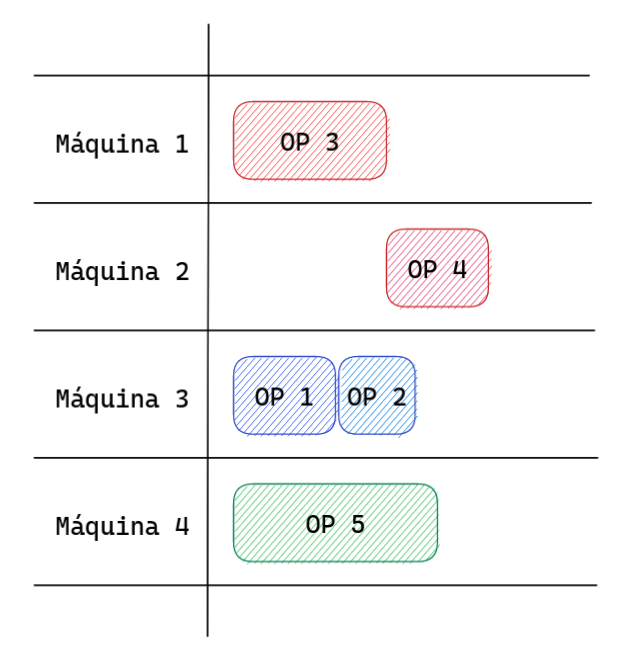
\includegraphics[scale=0.43]{ejemplo.png}
    \caption{Posible solución del ejemplo mostrado.}
    \label{fig:example-solution}
\end{figure}

La distribución final de tiempos para cada máquina es la siguiente: 
\begin{itemize}
    \item \textbf{Máquina 1}, OP 3 (3 UT) + 0 GAP = 3 UT 
    \item \textbf{Máquina 2}, OP 4 (2 UT) + 3 GAP = 5 UT 
    \item \textbf{Máquina 3}, OP 1 (2 UT) + OP 2 (1 UT) + 0 GAP = 3 UT 
    \item \textbf{Máquina 4}, OP 5 (4 UT) + 0 GAP = 4 UT. 
\end{itemize}

Ya que el tiempo total de producción es el tiempo de finalización de la máquina más lenta, 
que es la máquina 2, son 5 UT o como se menciona en la literatura un makespan de 5.
Nótese que el gap de la máquina 2 es derivado de la dependencia
existente entre la operación 4 y la operación 3 por pertenecer ambos al trabajo B, 
por lo tanto, antes de que dicha maquina empiece con la operación 4 tiene que esperar 
a que se procese la máquina 1.

\subsection{Estructura del documento}
En esta sección, se presenta la estructura del documento de forma clara y organizada. Se 
brinda una visión general de cómo se han organizado los diferentes capítulos y secciones 
para abordar de manera coherente y completa todos los aspectos relevantes del proyecto. 
Además, se proporciona una breve descripción de cada capítulo, destacando su contenido 
y su contribución al conjunto de la memoria. Esta sección permite al lector tener una 
guía clara sobre cómo está estructurado el documento y qué puede esperar encontrar en cada 
sección.

\begin{itemize}
    \item \textbf{Introducción.} En este capítulo se presenta de forma breve el objetivo 
    principal del proyecto, su impacto deseado y la motivación detrás de su realización. 
    Además, se realiza una  breve descripción del problema a resolver y se enumeran de manera 
    ordenada los capítulos que componen el proyecto.
    \item \textbf{Antecedentes y justificación.} Se proporciona un estudio del estado del 
    arte y las últimas tendencias, y se justifican las antecedentes existentes durante el 
    desarrollo del proyecto.
    \item \textbf{Alcance y objetivos.} Se definen de manera detallada tanto el objetivo 
    principal como los objetivos secundarios del proyecto. También se establece el alcance 
    del proyecto, que se describe mediante una lista concisa de elementos que se encuentran 
    dentro y fuera del proyecto.
    \item \textbf{Metodología.} Se describe la metodología de trabajo utilizada durante el
    desarrollo del proyecto, así como la metodología creada para la resolución del problema.
    \item \textbf{Memoria técnica.} Se explican en detalle todos los aspectos técnicos del mismo. 
    Se incluyen la arquitectura del sistema integral, las herramientas utilizadas para el desarrollo, 
    los requisitos del sistema y las incidencias encontradas entre otros.
    \item \textbf{Proceso de desarrollo.} En este capitulo se presenta el proceso de desarrollo 
    utilizado en el proyecto. Se describe de manera detallada la metodología y las prácticas 
    empleadas durante la resolución del problema. Proporciona una visión general del enfoque 
    adoptado en el desarrollo del proyecto y cómo se aseguró la calidad y eficiencia en la 
    implementación del sistema. También se discuten posibles limitaciones de los métodos 
    y se proponen recomendaciones para investigaciones futuras.
    \item \textbf{Experimentación.} En este apartado se describe el proceso de experimentación 
    llevado a cabo en el proyecto. Se detallan los experimentos realizados, las diferentes
    representaciones del problema, los datos recopilados y los resultados obtenidos. Además, 
    se analizan e interpretan los resultados para sacar conclusiones relevantes y respaldar 
    las decisiones tomadas en el proyecto.  
    \item \textbf{Planificación y presupuesto.} Se detallan las fases y tareas del proyecto, se organizan 
    cronológicamente indicando su duración. También se incluye un esquema de descomposición 
    del trabajo y el plan de recursos humanos. Además, se incluyen los costes totales del proyecto, 
    incluyendo los materiales y los recursos humanos.
    \item \textbf{Conclusiones y trabajo a futuro.} Se presentan las reflexiones realizadas 
    tras la finalización del proyecto, así como las lecciones aprendidas y los conocimientos 
    adquiridos. Además, se presentan ideas o propuestas que podrían ser utilizadas o implementadas 
    en futuras investigaciones.
    \item \textbf{Abreviaturas, acrónimos y definiciones.} Se proporcionan explicaciones sobre 
    el significado de ciertos términos, acrónimos o abreviaturas mencionadas en la memoria y 
    que se consideran relevantes.
    \item \textbf{Bibliografía.} Se incluye una lista de referencias bibliográficas utilizadas
    durante el desarrollo de la memoria.
    \item \textbf{Anexos.} Se incluyen documentos independientes a la memoria del proyecto, 
    pero considerados lo suficientemente relevantes como para ser adjuntados en documentos separados.
    \begin{itemize}
        \item \textbf{Anexo I, Manual de usuario.} Se proporcionan las instrucciones necesarias 
        para que cualquier usuario, independientemente de su nivel de conocimiento sobre el tema 
        del proyecto, pueda poner en marcha el sistema inteligente y aprovechar todas sus funcionalidades.
        \item \textbf{Anexo II, Dimensión ética del proyecto.} Se realiza un análisis ético del proyecto 
        para garantizar que en su conjunto sea considerado éticamente aceptable y una contribución positiva 
        para la sociedad.
    \end{itemize}

\end{itemize}



\pagebreak